\chapter{Campus Topology}\label{ch:Design}

\section{A2.1 -- The Router Hunt}
Traceroutes were run to at least 10--15 destinations: campus services
(\texttt{www.iitd.ac.in}, \texttt{moodle}, \texttt{library}, \texttt{webmail},
\texttt{cse}, \texttt{am}, \texttt{chemical}, \texttt{design}, \texttt{dms}, \texttt{textile},
\texttt{ee}, \texttt{maths}) and external destinations (\texttt{1.1.1.1}, \texttt{8.8.8.8},
\texttt{www.iitb.ac.in}, \texttt{www.mit.edu}, and several large commercial sites used purely
to sample more of the egress path). Table~\ref{tab:hophunt} lists every distinct internal
(\texttt{10.x.x.x}) hop observed, an abbreviated view of which traces it appeared in, its
position along the path, its average RTT, and our best guess at its role, reasoned from that
position, recurrence, and RTT together.

\begin{table}[H]
\centering
\footnotesize
\caption{Observed internal hops and inferred roles. ``Traces'' is abbreviated to a representative
subset with a count; the full per-trace list for each hop is preserved as Evidence~E-2.}
\label{tab:hophunt}
\begin{tabular}{@{}p{2.1cm}p{4.1cm}ccp{3.9cm}@{}}
\toprule
Hop IP & Representative traces (count) & Pos. & Avg RTT (ms) & Best guess at role \\
\midrule
10.184.0.13 & www.iitd.ac.in, moodle, cse, 8.8.8.8, www.iitb.ac.in, \ldots\ (24) & 1 & 4.45 & Local gateway (T1) for the hostel area \\
10.254.236.26 & am, webmail, textile, dms, moodle, www.iitd.ac.in, design (7) & 2 & 5.09 & Primary aggregation router (campus services) \\
10.254.236.6 & ee, library, chemical, maths (4) & 2 & 4.55 & Secondary aggregation router \\
10.10.17.1 & moodle (1) & 3 & 3.62 & Department / service subnet gateway \\
10.254.208.6 & cse (1) & 2 & 7.17 & Department subnet gateway (CSE) \\
10.208.20.2 & cse (1) & 3 & 7.17 & Department subnet gateway (CSE, internal) \\
10.10.211.213 & am (1) & 3 & 8.44 & Department / service subnet gateway \\
10.7.10.101 & chemical (1) & 3 & 6.22 & Department / service subnet gateway \\
10.10.17.2 & design (1) & 4 & 6.13 & Department / service subnet gateway \\
10.10.211.211 & textile (1) & 3 & 7.51 & Department / service subnet gateway \\
10.10.211.216 & maths (1) & 3 & 4.96 & Department / service subnet gateway \\
10.255.109.100 & whatsapp, amazon, instagram, google, netflix, mit.edu, \ldots\ (15) & 2 & 5.01 & Campus core distribution router \\
10.255.107.3 & (as above) + www.iitb.ac.in (16) & 3 & 5.39 & Campus core distribution router \\
10.119.233.65 & (as above) (16) & 4 & 5.99 & Internal border / transit router \\
10.119.234.162 & amazon, ibm, netflix, mit.edu, wikipedia, x, microsoft, reddit, apple (9) & 6 & 8.55 & External egress gateway (commercial ISP path) \\
10.1.207.69 & whatsapp, instagram, iitb.ac.in, google, facebook, 8.8.8.8 (6) & 5 & 29.22 & Transit router (NKN / peering path) \\
10.1.200.137 & whatsapp, instagram, iitb.ac.in, google, facebook, 8.8.8.8 (6) & 6 & 34.58 & Transit router (NKN / peering path) \\
\bottomrule
\end{tabular}
\end{table}

\textcolor{red}{\footnotesize Note: position/RTT reconstructed from a flattened source table -- verify against the original CSV before final submission (likely viva material).}

A few observations follow directly from the table. \texttt{10.184.0.13} appears at position~1 in
every trace we ran -- consistent with it being our own default gateway rather than a shared
campus device. The pair \texttt{10.255.109.100} / \texttt{10.255.107.3} / \texttt{10.119.233.65}
appears in every trace to an external commercial destination but never in traces to
\texttt{www.iitd.ac.in} or other campus services, which is the signature of a core/egress path
that campus-internal traffic never needs to cross. Two hops, \texttt{10.1.207.69} and
\texttt{10.1.200.137}, sit at a noticeably higher average RTT (29--35\,ms) than the rest of the
internal hops (4--9\,ms); combined with their appearing only on traces toward external
destinations and not toward \texttt{www.iitb.ac.in} exclusively, we read them as the
peering/transit hops just before or on IIT Delhi's connection to the National Knowledge Network
(NKN) or a commercial upstream, rather than anything internal to a single building. The
department gateways (\texttt{10.10.17.x}, \texttt{10.10.211.x}, \texttt{10.208.20.2},
\texttt{10.7.10.101}, \texttt{10.254.208.6}) each appeared in exactly one trace, which is
expected: each department's traceroute only crosses its own subnet gateway.

\subsection{Internal Topology Graph}
Figure~\ref{fig:topology} draws the internal topology as a graph, with routers as nodes and
observed adjacencies (which hop directly followed which, across all traces) as edges.

\begin{figure}[H]
    \centering
    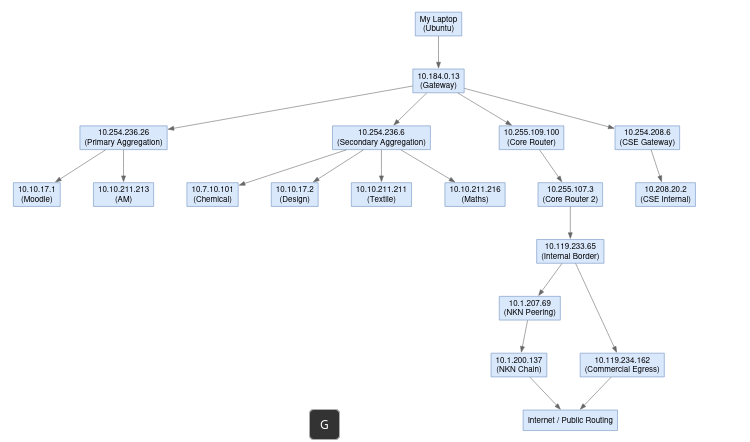
\includegraphics[width=0.85\textwidth]{report/images/a2_topology_graph.png}
    \caption[Internal topology graph]{Internal topology graph built from observed adjacencies in Table~\ref{tab:hophunt}. Edges represent a hop directly following another in at least one trace; nothing past the last labelled node was directly observed.}
    \label{fig:topology}
\end{figure}

\section{A2.2 -- The Wireless Layer}
A Wi-Fi survey was run from three locations on campus using \texttt{nmcli}, recording every
broadcast SSID together with its BSSID, band, channel, and signal strength.

\begin{table}[H]
\centering
\footnotesize
\caption{Wireless survey across three locations (redundant enterprise BSSIDs at Satpura truncated for length; full capture preserved as Evidence E-3).}
\begin{tabular}{@{}p{1.8cm}p{3.0cm}p{3.2cm}ccc@{}}
\toprule
Location & BSSID & SSID & Band & Ch. & Sig. \\
\midrule
Satpura & 4E:BC:FE:A5:A4:A4 & realme P2 Pro 5G & 2.4 GHz & 6 & 97 \\
Satpura & E4:4E:2D:0C:82:61 & eduroam & 2.4 GHz & 1 & 74 \\
Satpura & E4:4E:2D:0C:82:60 & IITD\_WIFI & 2.4 GHz & 1 & 74 \\
Satpura & E4:4E:2D:0C:82:64 & IITD\_Secure\_GUEST & 2.4 GHz & 1 & 74 \\
Satpura & E4:4E:2D:0C:82:63 & (Hidden) & 2.4 GHz & 1 & 74 \\
Satpura & E4:4E:2D:0C:82:6E & eduroam & 5 GHz & 44 & 70 \\
Satpura & E4:4E:2D:0C:82:6F & IITD\_WIFI & 5 GHz & 44 & 69 \\
Satpura & E4:4E:2D:0C:8B:E1 & eduroam & 2.4 GHz & 6 & 59 \\
Satpura & A4:B4:39:40:C3:61 & eduroam & 2.4 GHz & 11 & 59 \\
Satpura & A4:B4:39:33:7E:A4 & IITD\_Secure\_GUEST & 2.4 GHz & 11 & 40 \\
Satpura & 88:9C:AD:5A:43:41 & eduroam & 2.4 GHz & 11 & 29 \\
\midrule
Lecture Hall & 54:8A:BA:DD:7A:C1 & IITD\_Secure\_GUEST & 2.4 GHz & 6 & 97 \\
Lecture Hall & 54:8A:BA:DD:7A:C4 & IITD\_WIFI & 2.4 GHz & 6 & 87 \\
Lecture Hall & 54:8A:BA:DD:7A:C3 & IITD\_IOT & 2.4 GHz & 6 & 87 \\
Lecture Hall & 54:8A:BA:DD:7A:CE & IITD\_Secure\_GUEST & 5 GHz & 36 & 82 \\
Lecture Hall & 04:5F:B9:2F:24:C1 & IITD\_Secure\_GUEST & 2.4 GHz & 1 & 69 \\
Lecture Hall & 70:BD:96:6E:75:42 & eduroam & 2.4 GHz & 11 & 65 \\
Lecture Hall & 38:7A:CC:6D:56:A9 & 3E4C54F42B90 & 5 GHz & 44 & 59 \\
Lecture Hall & 78:22:88:40:9F:42 & 454B10749644 & 5 GHz & 44 & 44 \\
Lecture Hall & 04:5F:B9:2F:24:CB & IITD\_WIFI & 5 GHz & 116 & 42 \\
\midrule
Library & 70:DF:2F:04:98:62 & eduroam & 2.4 GHz & 1 & 72 \\
Library & 70:DF:2F:04:98:63 & IITD\_IOT & 2.4 GHz & 1 & 72 \\
Library & 5C:A6:2D:44:E7:E2 & eduroam & 2.4 GHz & 11 & 62 \\
Library & 5C:A6:2D:44:E7:ED & eduroam & 5 GHz & 128 & 56 \\
Library & 70:DF:2F:04:98:6C & IITD\_IOT & 5 GHz & 149 & 52 \\
Library & B8:B7:DB:E6:BD:B5 & 26582626 & 2.4 GHz & 5 & 42 \\
Library & BE:00:19:A0:0C:FA & rjnish & 2.4 GHz & 6 & 40 \\
Library & 5C:A6:2D:6F:F8:E1 & IITD\_Secure\_GUEST & 2.4 GHz & 1 & 39 \\
\bottomrule
\end{tabular}
\end{table}

\subsection{Reading the Survey}
\textbf{How many physical APs.} SSIDs are not access points -- a single radio commonly
broadcasts several SSIDs from one MAC block (multiple BSSID / MBSSID), differing only in the
last hex digit. Grouping BSSIDs by their shared prefix rather than counting SSID rows gives 5
distinct physical enterprise APs in Satpura, 3 in the Lecture Hall, and 4 in the Library --
noticeably fewer than the raw broadcast count.

\textbf{Global vs.\ localised SSIDs.} \texttt{eduroam}, \texttt{IITD\_WIFI}, and
\texttt{IITD\_Secure\_GUEST} appear in all three locations and are evidently provisioned
campus-wide. \texttt{IITD\_IOT} appears in both academic locations (Lecture Hall, Library) but
not once in the Satpura data, which reads as a deliberate choice to keep IoT infrastructure out
of residential buildings rather than a coverage gap -- though we cannot rule out that our single
Satpura vantage point simply missed an IITD\_IOT radio elsewhere in the hostel. Personal
hotspots (\texttt{realme P2 Pro 5G}, \texttt{rjnish}, the two unnamed hex-string SSIDs in the
Lecture Hall) are, as expected, seen at exactly one location each and nowhere else.

\textbf{Channel plan.} Across all three surveys, zero networks were observed on 2.4\,GHz
channels 3, 4, or 8 -- every enterprise AP sits on 1, 6, or 11, the three mutually
non-overlapping channels. This is consistent with the campus enforcing a fixed channel plan
(RRM) on managed infrastructure. The one exception is the student hotspot \texttt{26582626} in
the Library, broadcasting on channel 5, which does create adjacent-channel interference with
neighbouring channel-1 and channel-6 networks -- but since it is a personal device we cannot
scan or otherwise investigate further under the assignment's rules.

\section{A2.3 -- The Class Map}
\textcolor{red}{\footnotesize TODO: add rows to \texttt{COL334\_A1\_Campus\_Map.xlsx}, verify two other teams' rows (confirmed/contradicted/couldn't reach), summarise here.}
